\documentclass[a4paper]{article}
\usepackage{hyperref}
\usepackage{subfigure}
\usepackage{titling}
\usepackage{listings}
\usepackage{color}
\usepackage{adjustbox}
\usepackage{graphicx}%,showframe
\graphicspath{ {img/} }
\definecolor{dkgreen}{rgb}{0,0.6,0}
\definecolor{gray}{rgb}{0.5,0.5,0.5}
\definecolor{mauve}{rgb}{0.58,0,0.82}

\lstset{frame=tb,
  aboveskip=3mm,
  belowskip=3mm,
  showstringspaces=false,
  columns=flexible,
  basicstyle={\small\ttfamily},
    numbers=left,                    
    numbersep=5pt,
  keywordstyle=\color{blue},
  commentstyle=\color{dkgreen},
  stringstyle=\color{mauve},
  breaklines=true,
  breakatwhitespace=true,
  tabsize=3
}

\title{%
    \textbf{Planning and Automated Reasoning - Automated Reasoning} \\ 
    \large \textbf{ \\ Implementation of the Congruence Closure Algorithm}}

\author{Andrea Mangrella - VR490856}

\begin{document}

\maketitle
\section{Introduction}
The congruence closure algorithm is an important method used in automated reasoning and symbolic computation to reason and solve equations and inequalities involving congruence relations. 

\noindent
The algorithm's primary objective is to determine if a set of equations and inequalities is simultaneously satisfiable (i.e., whether there exists an assignment of values to the variables that satisfies all the given equations and inequalities). More specifically it focuses on reasoning about congruence relations, which are equivalence relations that preserve the structure of the underlying operations. Congruence Closure is commonly employed in various fields, like theorem proving and program analysis.

\section{Project Structure}
I decided to implement the project in Python3, mainly because it's the language I'm most familiar with and there are a multitude of open source libraries on pypi, furthermore pip is a decent package manager.
I used python modules to organize the repository, the module is stored in the \textit{lib} directory and contains the following files:
\begin{itemize}
    \item  \textit{smt\_parse.py}: this file contains a function to parse smt files using the pysmt package, it also splits the parsed formulas (that have to be already in DNF) first on OR clauses, and then on AND clauses. 
    \item \textit{general\_parsing.py}: contains the class parse\_atoms function that builds the DAG and the parse\_equations function that transforms equations and inequalities in id tuples.
    \newpage
    \item \textit{congruence\_closure.py}: contains the \textit{CC\_DAG} class, nodes are stored using a networkx\footnote{https://networkx.org/} that works as a dictionary with node IDs as keys and other dictionaries as values, these dictionaries contain all of the nodes information. This class contains all the standard function from the book (reported below) and some utility functions like the graph drawing function (that uses networkx and matplotlib) and the string function that, by using recursion, from a node id generates a string alike to the one found during parsing. 
\end{itemize}
\subsection{Congruence Closure Class}

\noindent
Like suggested in the textbook\footnote{Aaron R. Bradley - Zohar Manna, The Calculus of Computation} I implemented the following functions:
\begin{itemize}
    \item \textit{NODE}
    \item \textit{Find}
    \item \textit{CCPAR}
    \item \textit{Congruent}
    \item \textit{Union} 
    \item \textit{Merge}
\end{itemize}
\subsection{Solve}
The solve function is the main cycle of the congruence closure algorithm and it cycles trough id pairs that represent equations or inequalities:
\begin{itemize}
    \item \textbf{Equations:} when first cycles trough equations pairs it checks if the two congruence classes (FIND attribute) are the same, if not it calls the \textit{Merge function}.
    \item \textbf{Inequalities:} the second cycle checks if the two congruence classes are not the same, indeed, if they are the algorithm returns UNSAT. If no inequality breaks this condition the algorithm returns SAT.
\end{itemize}
\begin{lstlisting}[language=Python,escapeinside={(*}{*)}, caption=The main function (with forbidden list) ]
    def solve(self):
        for eq in self.equalities:
            # Forbidden List  
            if (eq in self.inequalities) or (eq[::-1] in self.inequalities): return "UNSAT (Forbiddend List)"
            # Call a merge on every Equality 
            self.merge(eq[0],eq[1])
        for ineq in self.inequalities:
            val1, val2 = self.find(ineq[0]), self.find(ineq[1])
            if val1 == val2: # If the inequality is not correct it's UNSAT 
                return "UNSAT"
        return "SAT"
\end{lstlisting}
\newpage
\noindent
As requested in the project description I added the \textit{forbidden list} to the Solve function: 
if any equality id pair can is also found inside the inequalities array the algorithm returns UNSAT on the spot.

\subsection{Union}
Union is the function in which the mutable parameters (FIND and CCPAR) are \textbf{changed}. FIND represents the congruence class of a node and CCPAR the father of a node. By using union on two nodes the function merges the two CCPAR's into one (deleting the second node CCPAR) and assigns it to the first node, then it assigns the the FIND attribute of the first node to the second one.

\noindent
The original union method has been updated with \textit{non arbitrary choice of the representative of new class} (as requested in the project description): the function checks wich of the two nodes has the bigger CCPAR and always merges the smaller CCPAR to the bigger one. 
\begin{lstlisting}[language=Python,caption=Union function (with Priority)]
    def union(self,id1,id2):
        n1 = self.NODE(self.find(id1))
        n2 = self.NODE(self.find(id2))
        if len(n2["mutable_ccpar"]) >= len(n1["mutable_ccpar"]):
            n1["mutable_find"]  = copy.copy(n2["mutable_find"])
            n2["mutable_ccpar"].update(n1["mutable_ccpar"])
            n1["mutable_ccpar"] = set()
        else:
            n2["mutable_find"]  = copy.copy(n1["mutable_find"])
            n1["mutable_ccpar"].update(n2["mutable_ccpar"])
            n2["mutable_ccpar"] = set()
\end{lstlisting}

\subsection{SMT\_parse}
In this function we parse a SmtLib file given as input (the input has to be in DNF) and obtain a formula, then we remove all brackets and split the resulting formula first on OR clauses, and then on AND clauses. 

\noindent
The ouput of this function are the following two lists:
\begin{itemize}
    \item The first is a list of lists, containing all the \textit{equations and inequalities} for each congruence closure algorithm call.
    \item The second list contains a set (so no dupes) of all the \textit{atoms} that appear in the equations and inequalities, these atoms are used to build the Directed Acyclic Graph used by the algorithm.
\end{itemize}
\noindent

\subsection{Rec build}
This function parses an atom recursively, and builds Graph nodes starting from the literals, then it creates nodes for the predicates when climbing up the recursive chain, and adding the already parsed nodes ids to the args field of the predicate. The functions checks if the nodes already exists using a default-dictionary\footnote{https://docs.python.org/3/library/collections.html}, before creating a dupe.

\subsection{Parse\_equations}
This function sorts the formula into two lists: equations and inequalities. It also parses the formula string and transforms it in a tuple containing the ids of the two operands. 

\section{Inputs}\label{sec:input}
I used the SmtLib standard of files as the primary and only choice of input for the algorithm.
SmtLib (Satisfiability Modulo Theories Library) is a standardized format and language for specifying and interacting with Satisfiability Modulo Theories (SMT) solvers, it's a framework that combines elements of propositional logic (SAT) with background theories, such as arithmetic, arrays, equalities, to solve complex decision problems. 

\noindent
The SmtLib language provides a standard syntax and semantics for expressing logical formulas and constraints in a machine-readable format, which is always good for parsing.
\begin{lstlisting}[caption=Example of a SmtLib file, label={lst:smt}]
(set-info :smt-lib-version 2.6)
(set-logic QF_UF)
(set-info :source |
Source: The calcolus of computation (Bradley-Manna) 
Translator: Andrea Mangrella. |)
(set-info :category "crafted")
(set-info :status unsat)
(declare-sort S1 0)
(declare-fun a () S1)
(declare-fun b () S1)
(declare-fun f (S1 S1) S1)
(assert (let ((t1 (f a b))(t2 (f t1 b )))(and (= t1 a) (not (= t2 a)))))
(check-sat)
(exit)
\end{lstlisting}

\section{Outputs}
The two images below represent the DAG before and after the Congruence Closure algorithm:
\begin{figure}[]
    \begin{adjustbox}{max width=1.2\linewidth,center}
    
        \subfigure[DAG before the algorithm, with only the CCPAR edges]{\label{subfig:i2_pre}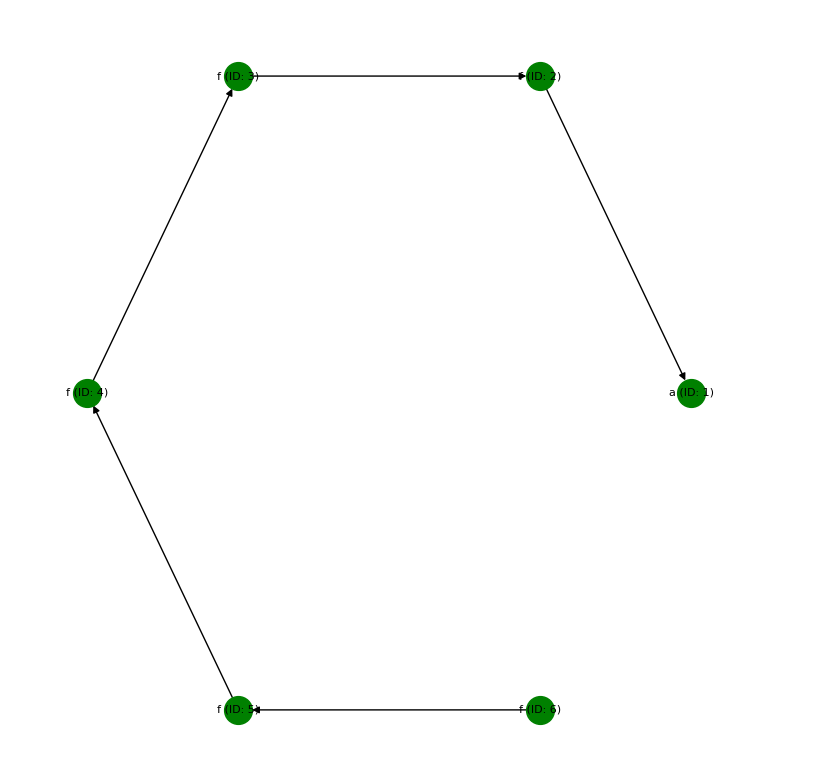
\includegraphics[width=0.55\textwidth]{images/pre.png}}%
        \subfigure[DAG processed with also the new FIND edges]{\label{subfig:i2_post}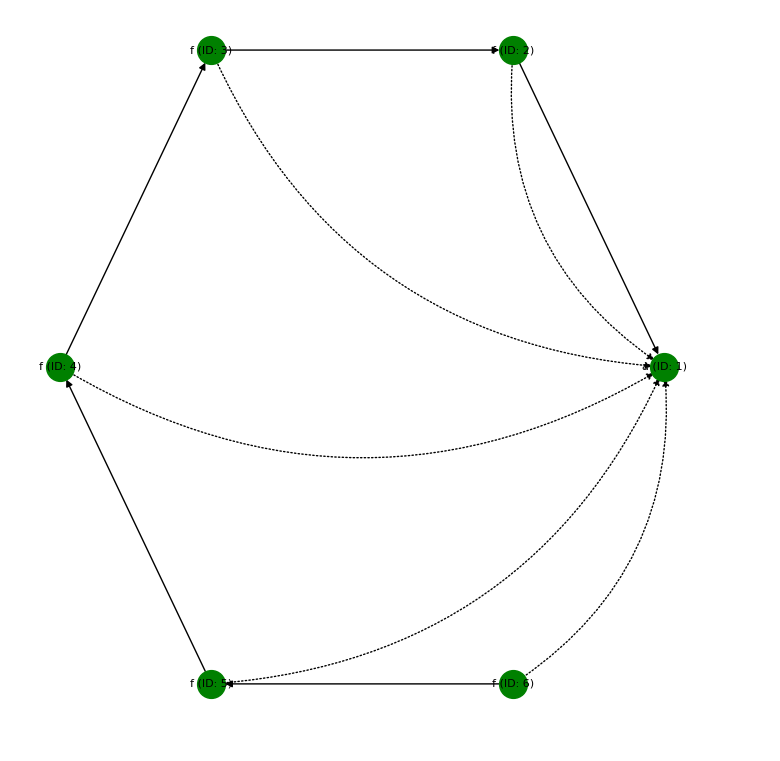
\includegraphics[width=0.55\textwidth]{images/post.png}}%

    \end{adjustbox}
    \label{fig:DAG}
    \caption{MatPlotLib graphs of a Directed Acyclic graph before and after Congruence Closure}
\end{figure}
\newpage
\noindent
The following block of text is an example of the output. It shows atoms, formulas, execution time and the result:
\begin{lstlisting}[caption=Result example]
File: ./ar_inputs/input1.smt2
Atoms:
['f(a, b)', 'a', 'f(f(a, b), b)']

Formulas:
['(f(a, b) = a)', '(! (f(f(a, b), b) = a))']
CC_DAG Result: UNSAT

FINAL RESULTS:
Ground Truth: UNSAT
End Result: UNSAT
Compilation Time: 0.00536
\end{lstlisting}

\newpage
\noindent
When using the \textbf{installer.sh} bash script in the project directory the executable will run on each one of the provided inputs, and the output for each one of them will be saved inside the \textbf{outputs directory}. The \textit{output} files also contain the total execution time for the given input.
\section{Conclusion}
The project works well with simple inputs already in DNF form. The first upgrade I would do is a DNF converter for the inputs, the reason why this would drastically improve the number of inputs is that SmtLib is a language written for solvers, and solvers usually take CNF formulas as inputs. As a matter of fact almost all of the inputs suggested in the project file\footnote{https://clc-gitlab.cs.uiowa.edu:2443/SMT-LIB-benchmarks/QF\_UF/-/tree/master} are in CNF. 

\end{document}